\documentclass[tikz,border=3pt]{standalone}
\usepackage[utf8]{inputenc}
\usepackage[T1]{fontenc}
\usepackage{lmodern}
\renewcommand{\familydefault}{\sfdefault}
\usepackage{sansmath}\sansmath
\usepackage{chemfig}
\usepackage{pgfplots}\pgfplotsset{compat=1.18,/pgf/number format/use comma,/pgf/number format/1000 sep={.}}
\usetikzlibrary{arrows.meta,calc,positioning,decorations.pathmorphing,patterns}
% paleta del sitio
\definecolor{nar}{HTML}{E8680C}\definecolor{narc}{HTML}{FFB35C}\definecolor{hielo}{HTML}{FFF3E8}
\definecolor{tinta}{HTML}{1D1D1F}\definecolor{gris}{HTML}{6E6E73}\definecolor{lila}{HTML}{7C5CF0}
\definecolor{azul}{HTML}{2F6FD6}\definecolor{menta}{HTML}{17A673}\definecolor{coral}{HTML}{E8342A}
\begin{document}
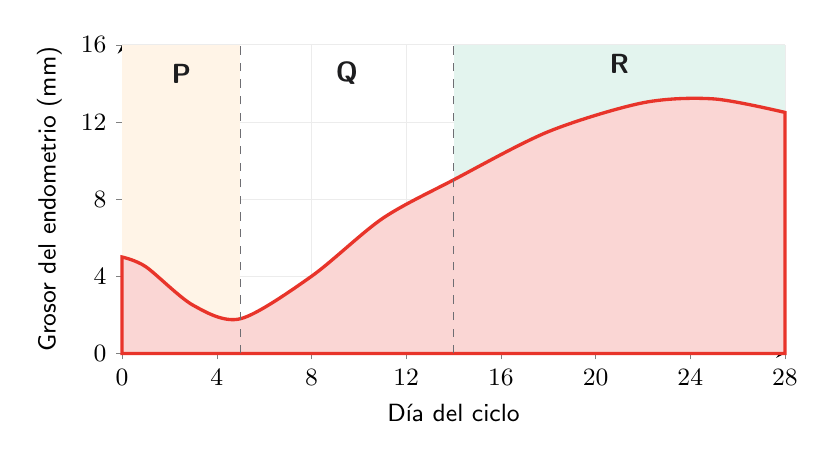
\begin{tikzpicture}[font=\small]
\begin{axis}[width=10cm,height=5.5cm,xmin=0,xmax=28,ymin=0,ymax=16,axis lines=left,xtick={0,4,...,28},ytick={0,4,8,12,16},
 xlabel={Día del ciclo},ylabel={Grosor del endometrio (mm)},grid=major,grid style={gray!15},clip=false]
\fill[narc!15] (axis cs:0,0) rectangle (axis cs:5,16);
\fill[menta!12] (axis cs:14,0) rectangle (axis cs:28,16);
\addplot[coral,very thick,smooth,fill=coral!20] coordinates {(0,5)(1,4.5)(3,2.5)(5,1.8)(8,4)(11,7)(14,9)(18,11.5)(22,13)(25,13.2)(28,12.5)} \closedcycle;
\node[font=\bfseries,text=tinta] at (axis cs:2.5,14.5) {P};
\node[font=\bfseries,text=tinta] at (axis cs:9.5,14.5) {Q};
\node[font=\bfseries,text=tinta] at (axis cs:21,15) {R};
\draw[gris,dashed] (axis cs:5,0) -- (axis cs:5,16) (axis cs:14,0) -- (axis cs:14,16);
\end{axis}
\end{tikzpicture}
\end{document}
